\documentclass[tikz,border=3.14mm]{standalone}
\usepackage{tikz}
\usetikzlibrary{calc}

\begin{document}

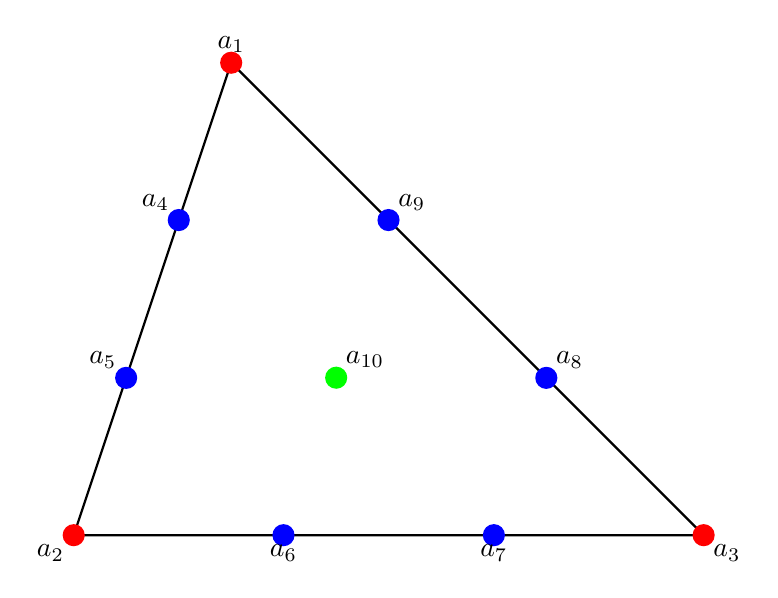
\begin{tikzpicture}[scale=2]

% 定义三角形顶点
\coordinate (A) at (0,0);
\coordinate (B) at (4,0);
\coordinate (C) at (1,3);

% 绘制三角形
\draw[thick] (A) -- (B) -- (C) -- cycle;

% 计算边上的三等分点
% AB边
\coordinate (AB1) at ($(A)!0.333!(B)$);
\coordinate (AB2) at ($(A)!0.667!(B)$);

% BC边  
\coordinate (BC1) at ($(B)!0.333!(C)$);
\coordinate (BC2) at ($(B)!0.667!(C)$);

% CA边
\coordinate (CA1) at ($(C)!0.333!(A)$);
\coordinate (CA2) at ($(C)!0.667!(A)$);

% 正确计算重心(三个顶点的平均值)
\coordinate (Int) at (barycentric cs:A=1,B=1,C=1); % 重心坐标

% 绘制顶点 (3个)
\fill[red] (A) circle (2pt);
\fill[red] (B) circle (2pt);
\fill[red] (C) circle (2pt);

% 绘制边上的点 (6个)
\fill[blue] (AB1) circle (2pt);
\fill[blue] (AB2) circle (2pt);
\fill[blue] (BC1) circle (2pt);
\fill[blue] (BC2) circle (2pt);
\fill[blue] (CA1) circle (2pt);
\fill[blue] (CA2) circle (2pt);

% 绘制内部点 (1个)
\fill[green] (Int) circle (2pt);

% 添加标签
\node[above] at (C) {$a_1$};
\node[below left] at (A) {$a_2$};
\node[below right] at (B) {$a_3$};

% 边上的点标签
\node[above left] at (CA1) {$a_4$};
\node[above left] at (CA2) {$a_5$};
\node[below] at (AB1) {$a_6$};
\node[below] at (AB2) {$a_7$};
\node[above right] at (BC1) {$a_8$};
\node[above right] at (BC2) {$a_9$};
% 内部点标签
\node[above right] at (Int) {$a_{10}$};


\end{tikzpicture}

\end{document}